% Chapter 2: State of the Art

\chapter{Tecnologías utilizadas} % Main chapter title

\label{Chapter2} % For referencing this chapter elsewhere, use \ref{Chapter2}

%-------------------------------------------------------------------------------

\section{Python}\label{sec:python}

Python\index{Python} es un lenguaje de programación orientada a objetos de alto nivel. Fue desarrollado originalmente por Guido van Rossum en el final de la década de 1980, y actualmente es gestionado por la \emph{Python Software Foundation} bajo una licencia \emph{open source}\index{open source} propia conocida como PSFL (\emph{Python Software Foundation License}). \emph{\parencite{Reference1}}

\begin{figure}[ht]
    \centering
    
\includegraphics[width=0.3\textwidth]{Figures/python-logo}
    \decoRule
    \caption[Python (Logo)]{Logo de Python\index{Python} \emph{\parencite{Reference2}}}
    \label{fig:python-logo}
\end{figure}

Python\index{Python} es actualmente uno de los lenguajes de programación más populares. Esto se debe en gran parte a su modularidad, la cual permite agregar fácilmente nuevas piezas de código a aplicaciones ya desarrolladas. \emph{\parencite{Reference3}}

\subsection{Poetry}\label{sec:poetry}

Poetry\index{Poetry} es un gestor de paquetes y dependencias para Python\index{Python}. Entre sus características más destacadas se encuentra la generación de un fichero con la especificación exacta de dependencias (incluidas las dependencias de dependencias), lo que asegura instalaciones idénticas en diferentes entornos. \emph{\parencite{Reference6}}

Además de esto, Poetry\index{Poetry} incorpora la mayoría de reglas establecidas en PEP\footnote{PEP (\emph{Python Enhancement Proposal}) recoge y describe las principales guías y recomendaciones de la comunidad respecto a nuevas características y procesos para cualquier desarrollo con Python.}, como el uso del fichero \emph{pyproject.toml} para escribir la metainformación de los paquetes, o el uso del esquema \emph{major.minor.micro} para los identificadores de versión. \emph{\parencite{Reference6}}

%-------------------------------------------------------------------------------

\section{HTTP}

\emph{Hypertext Transfer Protocol} (HTTP\index{HTTP}) es un protocolo de nivel de aplicación para sistemas de información distribuidos.

Es un protocolo genérico y sin estado que es usado para múltiples tareas como la transferencia de hipertexto o la representación de sistemas de ficheros.

Una característica de HTTP\index{HTTP} es la negociación de la representación de los datos, lo que permite construir sistemas independientemente de los datos que se vayan a transmitir. \emph{\parencite{Reference26}}

\subsection{API REST}

Una API\index{API} (\emph{Application Programming Interface}) es un contrato entre dos equipos sobre como deben comunicarse entre ellos. Con el uso de APIs se pretende abstraer los detalles acerca de como un sistema funciona internamente, haciendo públicas solo aquellas partes que los desarrolladores pudieran encontrar interesantes. De hecho, aunque la lógica interna cambiara, la API debería permanecer intacta. \emph{\parencite{Reference27}}

REST\index{REST} (\emph{Representational State Transfer}) es un estilo de arquitecura \emph{software}\index{software} para sistemas distribuidos que operan con contenido de diverso tipo. La idea tras este estilo es que cada respuesta del servidor debe ser una representación de un recurso (comúnmente en formato JSON\index{JSON}), siendo las llamadas a este solicitudes para la creación, actualización o eliminación de un recurso. \emph{\parencite{Reference28}}

Por tanto, una API\index{API} REST\index{REST} sería aquella que sigue los principios arquitectónicos que le dan nombre.

%-------------------------------------------------------------------------------

\section{Django}\label{sec:django}

Django\index{Django} es un \emph{web framework} desarrollado para Python\index{Python} y que, al igual que este, cuenta con una licencia \emph{open source}\index{open source}. Fue desarrollado originalmente por Adrian Holovaty y Simon Willison, dos programadores web que trabajaban en un periódico. \emph{\parencite{Reference4}}

\begin{figure}[ht]
    \centering
    
\includegraphics[width=0.3\textwidth]{Figures/django-logo}
    \decoRule
    \caption[Django (Logo)]{Logo de Django\index{Django} \emph{\parencite{Reference5}}}
    \label{fig:django-logo}
\end{figure}

Django\index{Django} sigue los principios de modularidad que caracterizan a Python\index{Python}, además de incluir muchas otras características interesantes como un sistema de vistas, modelos y plantillas que permite agilizar el desarrollo de aplicaciones web. Esto, sumado a un servidor web simple para desarrollos locales, una interfaz administrativa intuitiva, y la posibilidad de construir \emph{middleware} de todo tipo, convierten a Django\index{Django} en uno de los \emph{frameworks} para desarrollo web más famosos y usados de los últimos años. \emph{\parencite{Reference4}}

\subsection{Django REST Framework}\label{sec:drf}

Django\index{Django} REST Framework (DRF) es un módulo para Django que amplía las características de este, y que facilita la creación de APIs REST manteniendo todas las ventajas de Django. \emph{\parencite{Reference7}}

\begin{figure}[ht]
    \centering
    
\includegraphics[width=0.5\textwidth]{Figures/drf-logo}
    \decoRule
    \caption[DRF (Logo)]{Logo de DRF \emph{\parencite{Reference8}}}
    \label{fig:drf-logo}
\end{figure}

A diferencia del \emph{framework} original, DRF se centra principalmente en la parte \emph{backend} que compone una aplicación web. Para ello, ofrece al usuario muchas más opciones para serializar la entrada y salida de datos, además de ampliar las conocidas \emph{Generic Views} de Django con mejoras relacionadas con la construcción de APIs. \emph{\parencite{Reference7}}

Permite además interaccionar fácilmente con la API construida a través de una interfaz web básica, y es capaz de generar documentación dinámica para la API siguiendo la especificación de OpenAPI\footnote{\url{https://spec.openapis.org/oas/v3.1.0}}. \emph{\parencite{Reference7}}

\subsection{Gunicorn}\label{sec:gunicorn}

Gunicorn\index{Gunicorn} (\emph{"Green Unicorn"}) es un servidor HTTP\index{HTTP}, escrito en Python\index{Python}, que implementa WSGI\footnote{WSGI (\emph{Web Server Gateway Interface}) establece cómo deben ser llevadas las peticiones del servidor web a la aplicación web escrita en Python, de manera síncrona. \emph{\parencite{Reference11}}} como protocolo de llamadas.

Funciona utilizando un esquema centralizado, donde un nodo maestro gestiona y orquesta diferentes tipos de nodos trabajadores. Estos pueden ser utilizados para procesar peticiones síncronas o asíncronas, y su número escala en función de la demanda que tenga el servidor. \emph{\parencite{Reference9}}

\begin{figure}[ht]
    \centering
    
\includegraphics[width=0.4\textwidth]{Figures/gunicorn-logo}
    \decoRule
    \caption[Gunicorn (Logo)]{Logo de Gunicorn \emph{\parencite{Reference10}}}
    \label{fig:gunicorn-logo}
\end{figure}

%-------------------------------------------------------------------------------

\section{GrimoireLab}\label{sec:grimoirelab}

GrimoireLab\index{GrimoireLab} es el resultado de años de investigación y análisis de comunidades \emph{open source}\index{open source} y procesos de desarrollo. Desarrollado originalmente por miembros del equipo \emph{LibreSoft} (que más tarde fundarían Bitergia), actualmente forma parte de CHAOSS, una iniciativa de la \emph{Linux Foundation} centrada en crear y modelar métricas sobre comunidades \emph{open source}\index{open source}. \emph{\parencite{Reference12}}

\begin{figure}[ht]
    \centering
    
\includegraphics[width=0.2\textwidth]{Figures/grimoirelab-logo}
    \decoRule
    \caption[GrimoireLab (Logo)]{Logo de GrimoireLab \emph{\parencite{Reference12}}}
    \label{fig:grimoirelab-logo}
\end{figure}

Se trata de un conjunto de herramientas diseñadas para recoger, enriquecer, consumir y visualizar datos de casi cualquier fuente relacionada con el desarrollo \emph{Open Source}\index{open source}.

Cada una de estas herramientas sirve a un propósito específico y, en su conjunto, proveen el servicio antes mencionado:

\begin{itemize}
    \item Perceval es el encargado de recoger los datos crudos de cada fuente de datos compatible con GrimoireLab\index{GrimoireLab}. Ya sea utilizando herramientas como Git\index{Git} o haciendo uso de la API\index{API} de la fuente analizada.
    \item GrimoireELK enriquece los datos recogidos por Perceval. Genera, a partir de estos, nuevos datos que son de interés para estudiar las comunidades \emph{open source}\index{open source}.
    \item Sorting Hat permite gestionar la información relacionada con identidades, incluso entre diferentes fuentes de datos.
    \item SirMordred es la herramienta orquestadora para GrimoireLab\index{GrimoireLab}. Se encarga de sincronizar a todas las componentes para dar servicio.
    \item ¡Y muchas más herramientas increíbles!
\end{itemize}

\begin{figure}[ht]
    \centering
    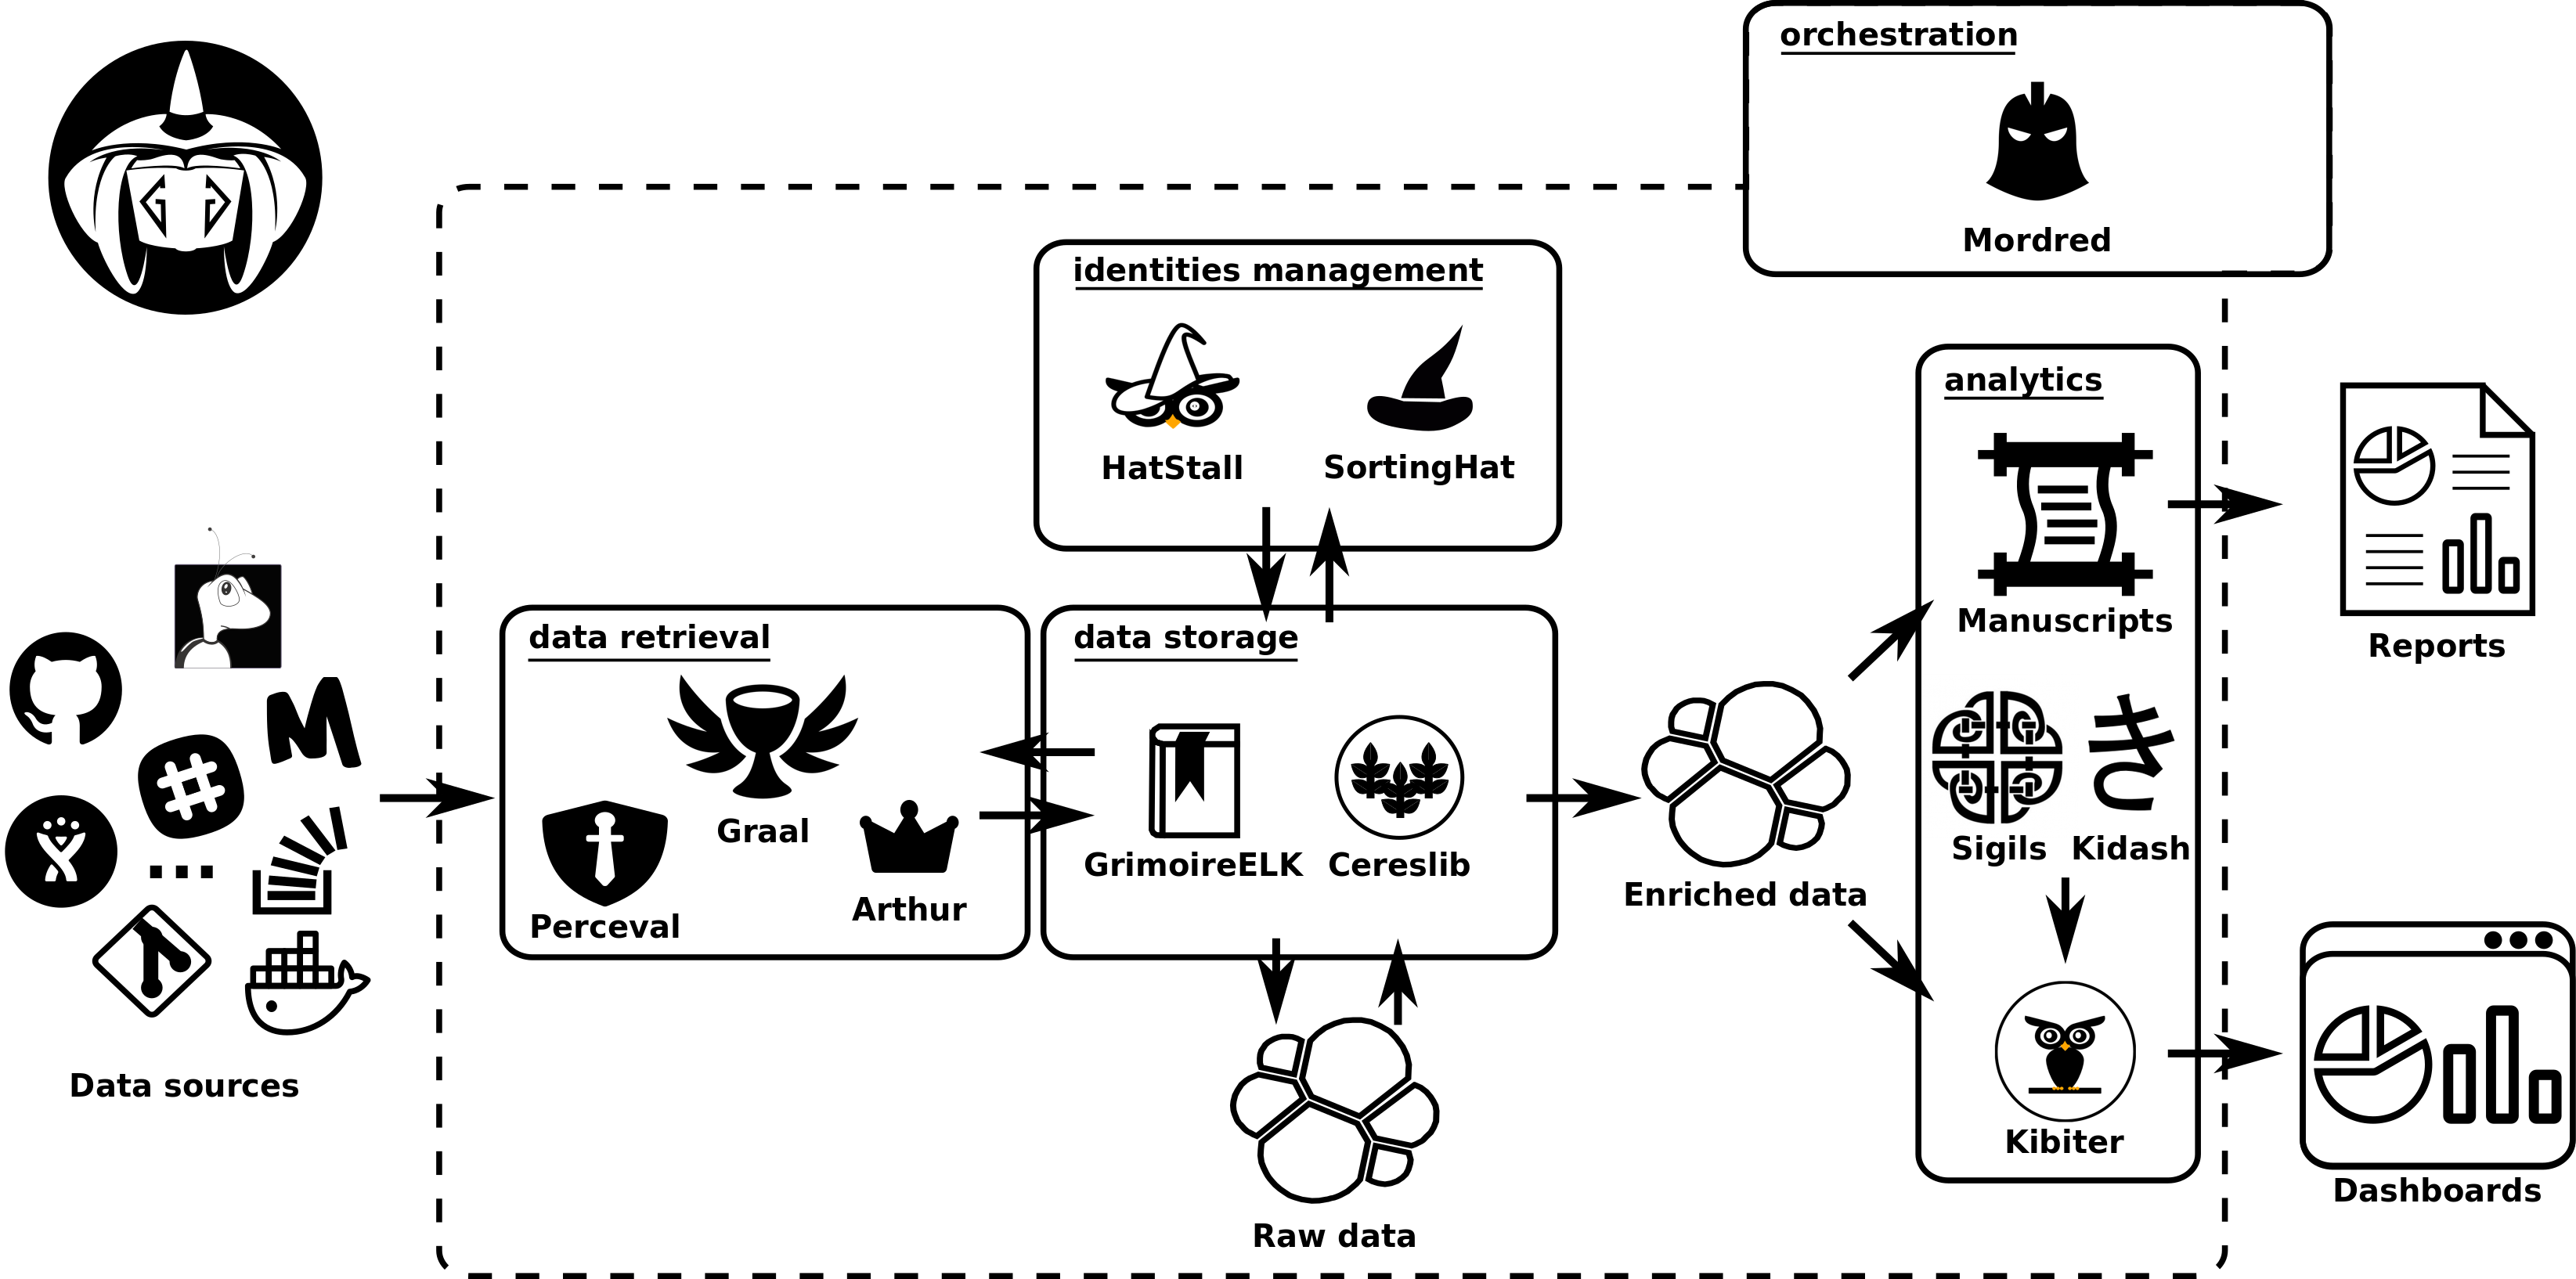
\includegraphics[width=0.7\textwidth]{Figures/grimoirelab-schema}
    \decoRule
    \caption[GrimoireLab (Esquema)]{Esquema de GrimoireLab \emph{\parencite{Reference12}}}
    \label{fig:grimoirelab-schema}
\end{figure}

\subsection{Cauldron.io}

Cauldron.io (o simplemente Cauldron\index{Cauldron}) es una plataforma web que permite a sus usuarios utilizar GrimoireLab\index{GrimoireLab} de manera sencilla y rápida, necesitando únicamente un navegador web para su uso. \emph{\parencite{Reference13}}

\begin{figure}[ht]
    \centering
    
\includegraphics[width=0.2\textwidth]{Figures/cauldron-logo}
    \decoRule
    \caption[Cauldron (Logo)]{Logo de Cauldron \emph{\parencite{Reference13}}}
    \label{fig:cauldron-logo}
\end{figure}

Cauldron\index{Cauldron} nace como un SaaS\footnote{\emph{Software as a Service}} de GrimoireLab\index{GrimoireLab}, y actualmente tiene compatibilidad con algunas de las fuentes de datos más importantes dentro de los ecosistemas \emph{open source}\index{open source}, como GitHub, Meetup, o StackExchange. Está compuesto por una aplicación Django\index{Django} detrás de un servidor Nginx, y utiliza Open Distro for Elasticsearch\index{Elasticsearch} y Kibana\index{Kibana} para almacenar y visualizar los datos generados con GrimoireLab\index{GrimoireLab}, respectivamente.

\begin{figure}[ht]
    \centering
    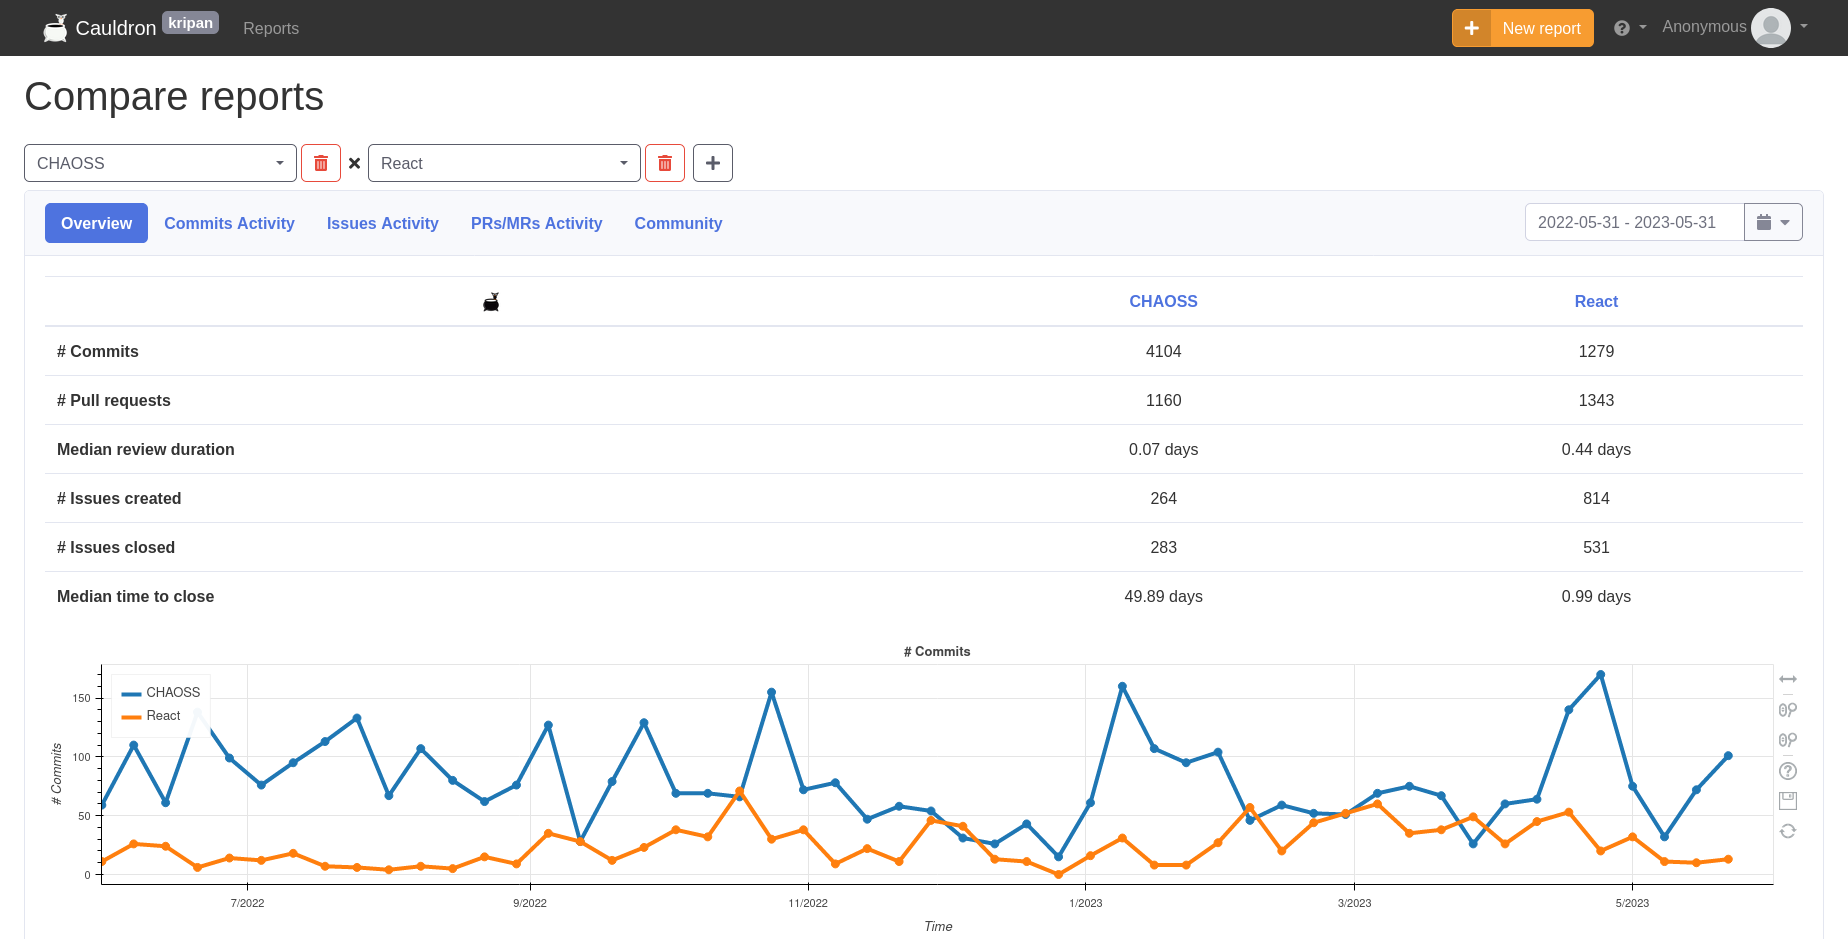
\includegraphics[width=\textwidth]{Figures/cauldron-charts}
    \decoRule
    \caption[Cauldron (Gráficas)]{Gráficas en Cauldron \emph{\parencite{Reference13}}}
    \label{fig:cauldron-charts}
\end{figure}

Además de las visualizaciones generadas en Kibana\index{Kibana}, Cauldron\index{Cauldron} ofrece a sus usuarios otras formas de dar valor a sus análisis. Como se observa en la Figura~\ref{fig:cauldron-charts}, permite comparar métricas y gráficas de diferentes proyectos. Además de esto, permite generar gráficas personalizadas dentro de Kibana\index{Kibana} gracias a las funcionalidades extra de Open Distro for Elasticsearch\index{Elasticsearch}.

%-------------------------------------------------------------------------------

\section{FastAPI}

FastAPI\index{FastAPI} es un \emph{web framework} desarrollado para Python\index{Python}, orientado principalmente a la construcción de APIs utilizando las anotaciones de tipos estándar de Python\index{Python}. \emph{\parencite{Reference14}}

\begin{figure}[ht]
    \centering
    
\includegraphics[width=0.7\textwidth]{Figures/fastapi-logo}
    \decoRule
    \caption[FastAPI (Logo)]{Logo de FastAPI \emph{\parencite{Reference14}}}
    \label{fig:fastapi-logo}
\end{figure}

FastAPI\index{FastAPI} nace después de que su autor no pudiera cubrir las necesidades de sus proyectos personales con los \emph{web frameworks} actuales en ese momento. Después de investigar las especificaciones de OpenAPI\index{OpenAPI}, JSON\index{JSON}, OAuth2, etc., decide construir su propia solución teniendo como base Pydantic\footnote{Pydantic es una herramienta que permite aprovechar las anotaciones de Python para informar de errores en la validación de datos.} y Starlette\footnote{Starlette es un framework que permite construir servicios web asíncronos en Python.}. \emph{\parencite{Reference15}}

FastAPI\index{FastAPI} hace uso de las anotaciones de tipos en Python\index{Python} para conseguir \emph{parsing} y validación de datos, documentación automática, y soporte en editores (comprobación de errores, autocompletado, etc). Hace uso de ASGI\footnote{ASGI (\emph{Asynchronous Server Gateway Interface}) es similar a WSGI, pero para llamadas asíncronas.} para llamadas asíncronas por defecto, es compatible con la mayoría de bases de datos relacionales y no relacionales, y permite tener un servicio web funcional en pocos pasos. \emph{\parencite{Reference14}}

\subsection{Uvicorn}

Uvicorn\index{Uvicorn} es un servidor HTTP\index{HTTP}, para aplicaciones Python\index{Python}, que procesa las llamadas de manera asíncrona implementando ASGI. En combinación con \nameref{sec:gunicorn}\index{Gunicorn}, se obtiene un servidor asíncrono multi nodo. \emph{\parencite{Reference16}}

\begin{figure}[ht]
    \centering
    
\includegraphics[width=0.3\textwidth]{Figures/uvicorn-logo}
    \decoRule
    \caption[Uvicorn (Logo)]{Logo de Uvicorn \emph{\parencite{Reference16}}}
    \label{fig:uvicorn-logo}
\end{figure}

%-------------------------------------------------------------------------------

\section{OpenSearch}\label{sec:opensearch}

OpenSearch\index{OpenSearch} es un \emph{suite} de herramientas \emph{open source}\index{open source} que permite el almacenamiento, búsqueda, y análisis de datos. Se trata de un proyecto formado principalmente por dos componentes: el propio motor OpenSearch\index{OpenSearch} y OpenSearch Dashboards, siendo estos un \emph{fork}\footnote{Uno de los principales motivos de su creación fue la decisión de modificar la licencia de Elasticsearch y Kibana a una no \emph{open source} por parte de sus creadores.} de los proyectos Elasticsearch\index{Elasticsearch} y Kibana\index{Kibana}, respectivamente. \emph{\parencite{Reference17}}

\begin{figure}[ht]
    \centering
    
\includegraphics[width=0.5\textwidth]{Figures/opensearch-logo}
    \decoRule
    \caption[OpenSearch (Logo)]{Logo de OpenSearch \emph{\parencite{Reference17}}}
    \label{fig:opensearch-logo}
\end{figure}

OpenSearch\index{OpenSearch} está basado en el motor de búsqueda Apache Lucene, lo que le confiere una gran capacidad de indexación en volúmenes de datos grandes. Muchas de las características que definen a OpenSearch\index{OpenSearch} provienen de plugins para Elasticsearch\index{Elasticsearch}, pero que el primero integra de manera nativa. Entre estas características destacan:

\begin{itemize}
    \item Un módulo avanzado de seguridad que permite la autenticación de usuarios mediante \emph{Active Directory}, LDAP, y otros protocolos similares. Igualmente, permite mayor granularidad sobre los permisos en índices y otras estructuras de datos.
    \item Un módulo de gestión de índices, con el que definir políticas y automatismos en índices.
    \item Un analizador de eficiencia que es capaz de obtener diversas métricas del \emph{cluster} de OpenSearch\index{OpenSearch} asociadas a la eficiencia, como la cantidad de memoria utilizada por los nodos, o el número de operaciones de lectura y escritura.
    \item Un sistema de alertas que permite establecer límites en gráficas y métricas, los cuales envían una notificación al ser rebasados.
\end{itemize}

\subsection{OpenSearch Dashboards}

OpenSearch\index{OpenSearch} Dashboards es la herramienta de visualización de datos de OpenSearch. Está basado en Kibana\index{Kibana}, tratándose de hecho de un \emph{fork} de esta. \emph{\parencite{Reference18}}

\begin{figure}[ht]
    \centering
    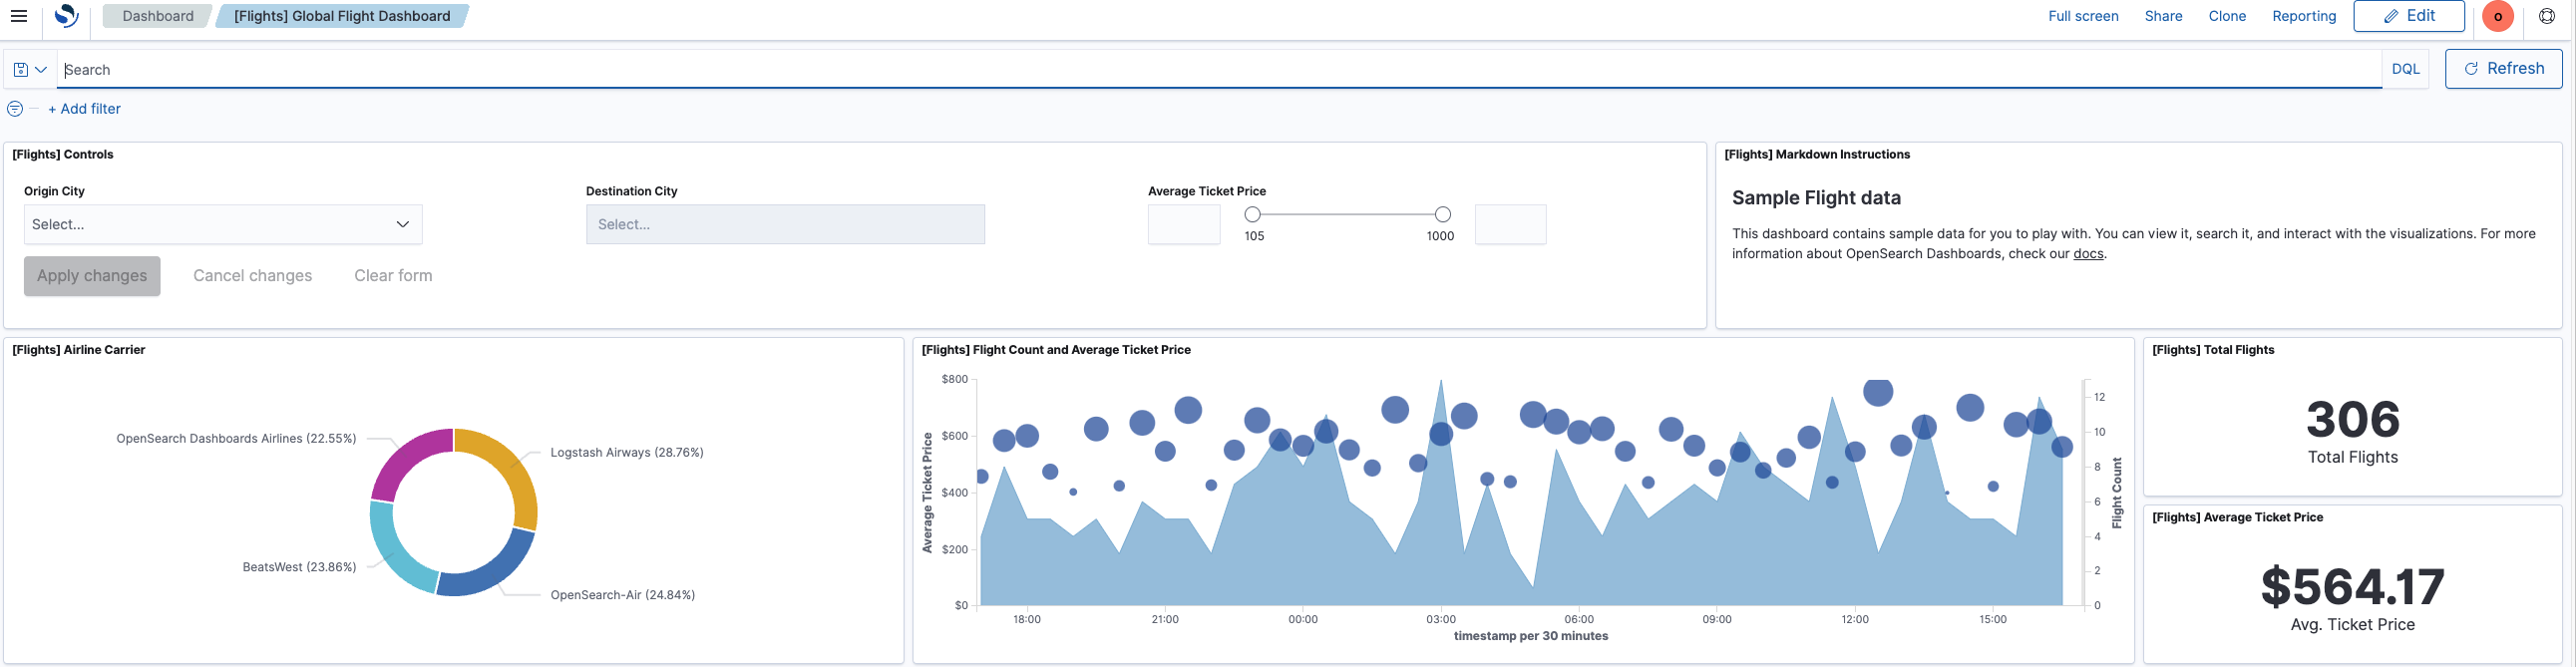
\includegraphics[width=\textwidth]{Figures/opensearch-dashboards}
    \decoRule
    \caption[OpenSearch Dashboards]{OpenSearch Dashboards \emph{\parencite{Reference18}}}
    \label{fig:opensearch-dashboards}
\end{figure}

Posee varias herramientas para interaccionar con los datos almacenados en el \emph{cluster} y crear, con estos, gráficos y métricas como los que aparecen en la Figura~\ref{fig:opensearch-dashboards}. Permite también la construcción de alias y patrones para índices, y la visualización de los datos directamente en formato JSON (tal y como están almacenados en el \emph{cluster}).

%-------------------------------------------------------------------------------

\section{PostgreSQL}

PostgreSQL\index{PostgreSQL} es un sistema de base de datos relacional con mucha historia (fue desarrollado originalmente en 1996). Cuenta con licencia \emph{open source}\index{open source}, y está gestionado por una comunidad colaborativa de desarroladores conocida como \emph{PostgreSQL Global Development Group}. \emph{\parencite{Reference19}}

\begin{figure}[ht]
    \centering
    
\includegraphics[width=0.3\textwidth]{Figures/postgresql-logo}
    \decoRule
    \caption[PostgreSQL (Logo)]{Logo de PostgreSQL \emph{\parencite{Reference19}}}
    \label{fig:postgresql-logo}
\end{figure}

PostgreSQL\index{PostgreSQL} es la opción recomendada para \nameref{sec:django}\index{Django}. Esto es debido a las muchas características que lo hacen una opción interesante, como la diversidad de estructuras nativas (\emph{arrays}, direcciones IP, etc), su capacidad para alta concurrencia, o la posibilidad de ejecutar bloques de código en el servidor.

%-------------------------------------------------------------------------------

\section{Docker}\label{sec:docker}

Docker\index{Docker} es el sistema gestor de contenedores\index{Contenedor} más utilizado actualmente, debido a la sencillez de su uso y a la cantidad de funcionalidades que ofrece. Docker\index{Docker} se basa en un esquema cliente-servidor donde el cliente es utilizado por los usuarios para comunicarse con el demonio de Docker\index{Docker} (el servidor), el cual se encarga de la construcción de contenedores\index{Contenedor}, su ejecución, y su distribución. \emph{\parencite{Reference20}}

\begin{figure}[ht]
    \centering
    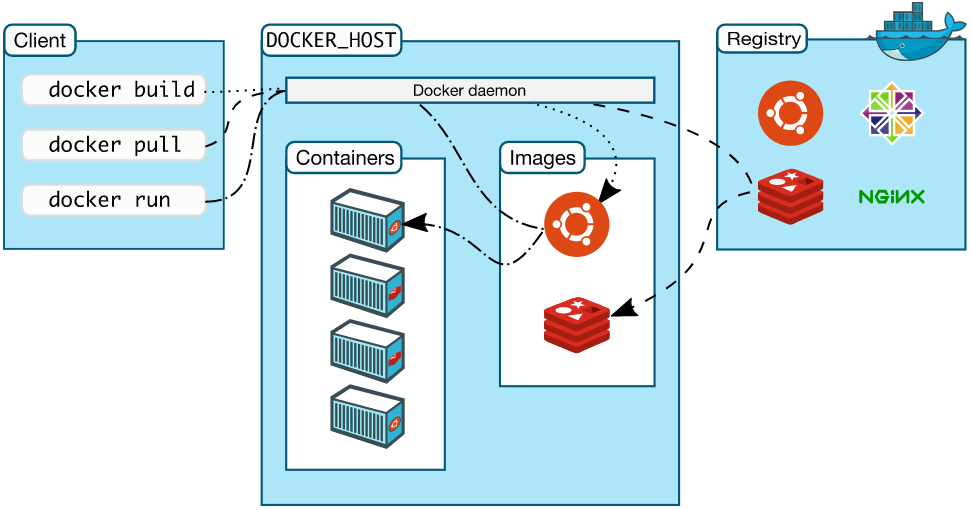
\includegraphics[width=0.8\textwidth]{Figures/docker-workflow}
    \decoRule
    \caption[Docker (\emph{Workflow})]{Flujo de trabajo en Docker \emph{\parencite{Reference20}}}
    \label{fig:docker-workflow}
\end{figure}

Como se observa en la Figura~\ref{fig:docker-workflow}, además del cliente y el demonio antes mencionados, en el despliegue y distribución de un contenedor\index{Contenedor} en Docker\index{Docker} intervienen varios elementos:

\begin{itemize}
    \item \textbf{Imágenes}: Una imagen en Docker\index{Docker} es una plantilla que detalla las instrucciones para la construcción de un contenedor\index{Contenedor}. Un usuario tiene la posibilidad de crear sus propias imágenes o utilizar las que otros usuarios hayan publicado en un registro. Para el primer caso, un usuario que quiera generar su propia imagen deberá crear un fichero \emph{Dockerfile} en el que se detallan las instrucciones (comandos) necesarias para la construcción del contenedor\index{Contenedor}.
    \item \textbf{Contenedores}: Un contenedor\index{Contenedor}, en Docker\index{Docker}, es una instancia ejecutable de una imagen. Pueden ser creados, iniciados, parados, o eliminados utilizando el cliente de Docker\index{Docker}. Se pueden conectar a una o más redes y se les puede agregar volúmenes para ampliar su espacio de almacenamiento.
    \item \textbf{Registros}: Un registro es un servidor donde los usuarios de Docker\index{Docker} pueden distribuir sus imágenes, de manera pública o privada.
\end{itemize}

%-------------------------------------------------------------------------------

\section{GitHub}

GitHub\index{GitHub} es un servicio \emph{online} que permite a los desarrolladores y a sus equipos llevar un control de versiones sobre sus proyectos \emph{software}\index{software}. Fue adquirido en 2018 por Microsoft y actualmente es la plataforma \emph{online} con mayor cantidad de repositorios de código del mundo. \emph{\parencite{Reference21}}

\begin{figure}[ht]
    \centering
    
\includegraphics[width=0.3\textwidth]{Figures/octocat}
    \decoRule
    \caption[Octocat]{Octocat (mascota de GitHub) \emph{\parencite{Reference23}}}
    \label{fig:octocat}
\end{figure}

GitHub\index{GitHub} es básicamente un SaaS de Git\index{Git}, pero con funcionalidades añadidas como la creación de \emph{issues} para el seguimiento de errores, la solicitud de cambios a código (conocidas como \emph{pull requests}), la inclusión de mecanismos automatizados (CI/CD), o la creación de \emph{wikis}, entre otros. \emph{\parencite{Reference22}}

\subsection{Dependabot}\label{sec:dependabot}

Dependabot\index{Dependabot} es una herramienta que permite a los desarrolladores despreocuparse de actualizar las dependencias de sus proyectos \emph{software}\index{software}. Se encarga de analizar los ficheros de dependencias de un proyecto\footnote{Por ejemplo, en un proyecto Python\index{Python} estas dependencias están definidas en el fichero \emph{requirements.txt} o \emph{pyproject.toml}.} y buscar nuevas actualizaciones de estas, notificando al usuario y, en ocasiones, sugiriendo los cambios necesarios al código para su inclusión. \emph{\parencite{Reference24}}

\begin{figure}[ht]
    \centering
    
\includegraphics[width=0.2\textwidth]{Figures/dependabot-logo}
    \decoRule
    \caption[Dependabot (Logo)]{Logo de Dependabot \emph{\parencite{Reference25}}}
    \label{fig:dependabot-logo}
\end{figure}

Dependabot\index{Dependabot} fue adquirido por GitHub\index{GitHub} en 2019, lo que ha permitido una integración más estrecha con la plataforma. Mediante la creación de un fichero \emph{dependabot.yml}, los desarrolladores pueden establecer que dependencias analizar, la frecuencia de estos análisis, y la fuente desde donde se buscan actualizaciones. \emph{\parencite{Reference24}}
